\section{\label{sec:SoA}Introduction}
Developing products, especially lightweight structures, 
requires a variety of steps from the original idea to the final product.
One approach to follow these steps for a successful production 
are described in the guidelines of VDI 2206 \cite{gausmeier2002} and VDI 2221 \cite{Jansch2006THEDO}.
These guidelines give a general methodology for designing technical systems and products, 
by introducing a methodical and systematic designing procedure, to work with maximum efficiency.
Since its first introduction in 1993, these guidelines have been applied within mechanical engineering, precision mechanics, 
switches and software development and the planning of process engineering \cite{pahl_beitz_2013}. 
Depending on the individual outcome, several steps might be repeated as part of a cyclic quality enforcing technique.
Especially in lightweight design the analysis, design and manufacturing processes are strongly connected, 
that they all have to be considered in every phase of the development process (Fig. \ref{pic:interactive-design}).
The amount of cyclic repeats is increasing simultaneously with higher demands on the products efficiency and error margin.
This fact causes it to be one of the main factors for increased development time.\\
\begin{figure}[h]
    \centering
    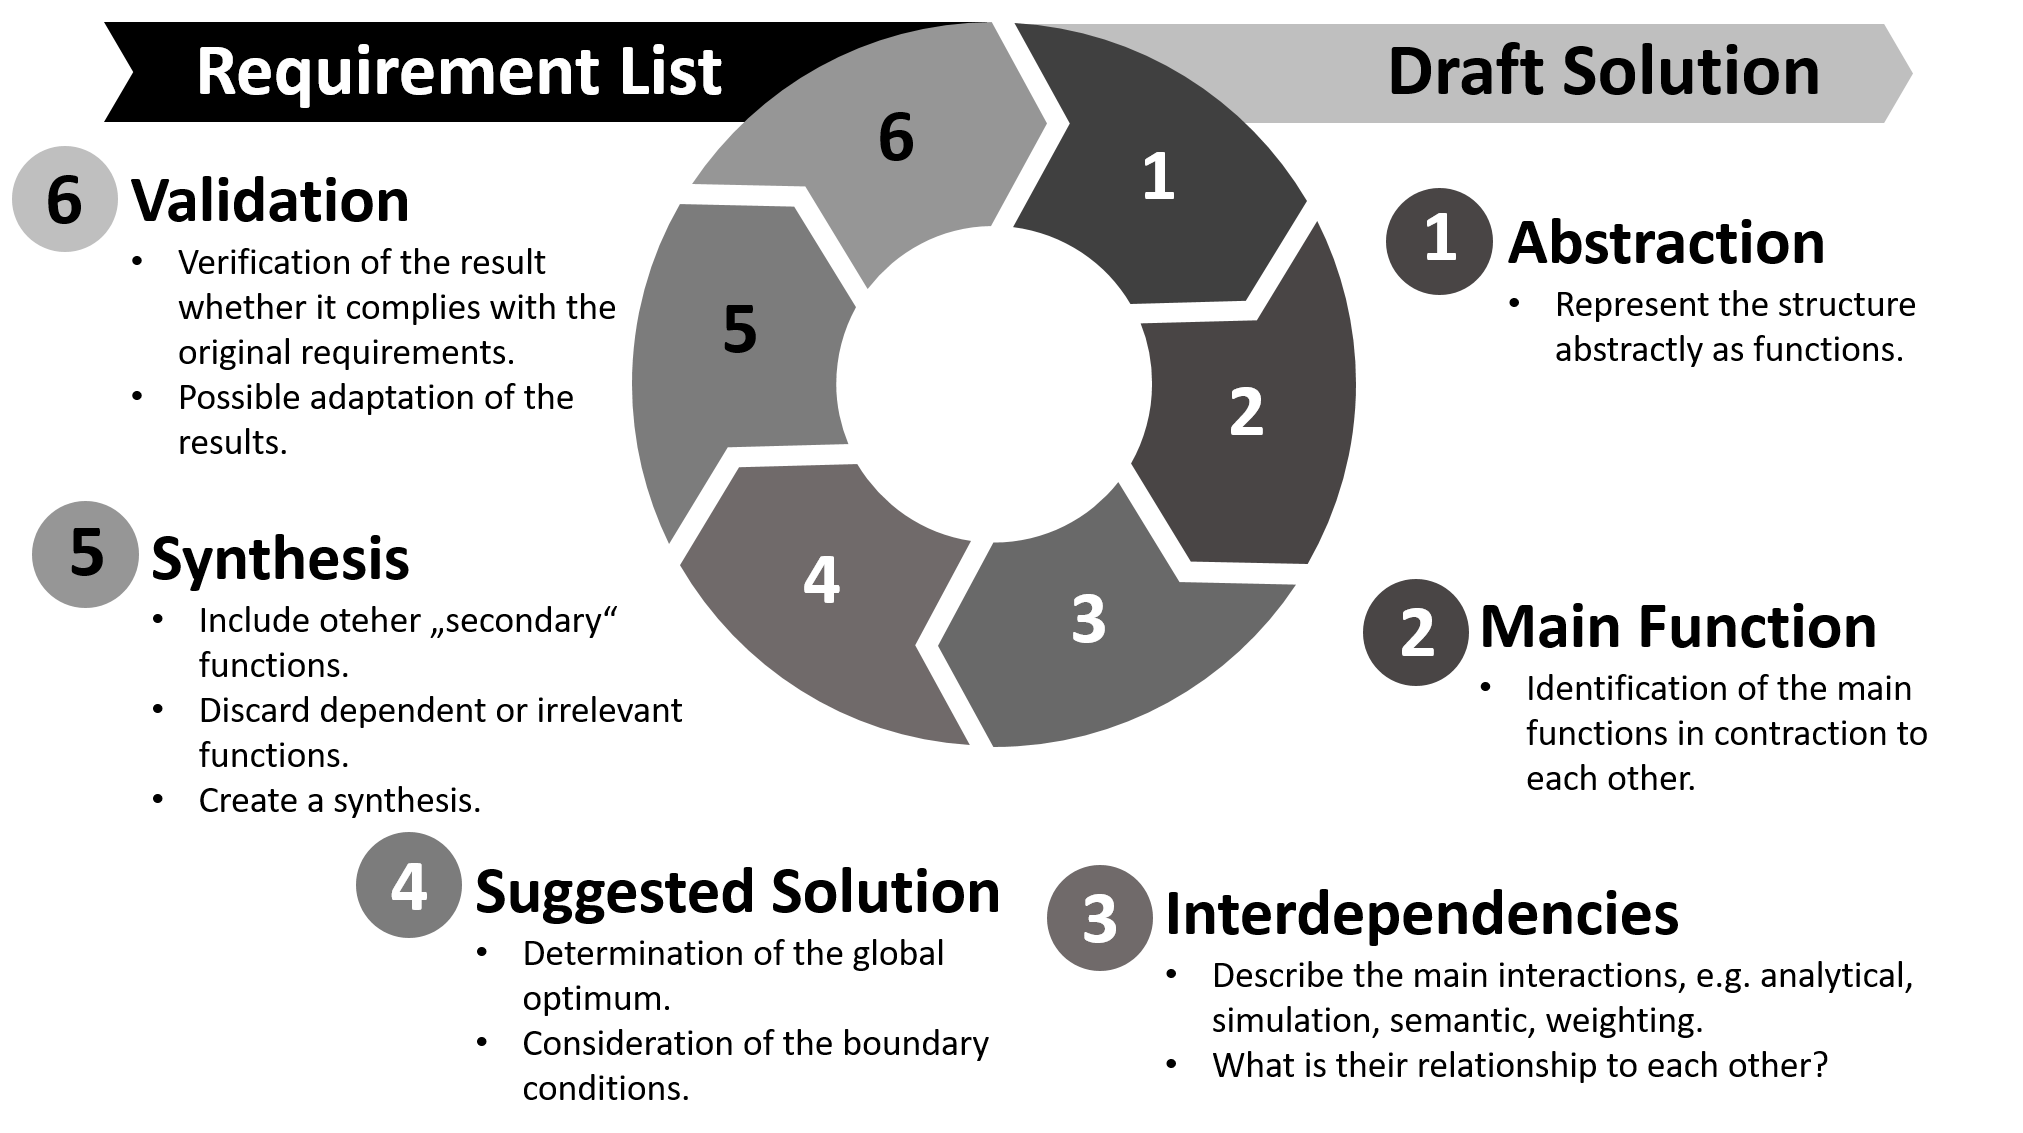
\includegraphics[scale=0.4]{pics/cyclic-design.PNG}
    \caption{\label{pic:interactive-design} A spiral development approach for complex function‐integrative lightweight systems. \cite{Modler2020}}
\end{figure}\\
Even before the rise of digital twins \cite{Leitenberger2021}, different solutions have been applied to digital represent each functionality and each dependencies of a system.
Starting in 1970, the fundament of current research on directed graphs was layed \cite{allen_control_1970}.
Today, solutions like ANSYS, SiemensNX, CAMUNDA, etc. implement workflow engines to automate processes which are presented as directed graphes \cite{noauthor_dynamo_2020, noauthor_function_2020, noauthor_systems_2020}.
These engines are build on certain requirements, like automating some of the simulation work and saving time by reusing models.\\
But these solutions lack certain capabilities, that makes same unsuited for multifunctional designs.
One reason for this is that no current system is capable of solving complex interactions over multiple domains,
as it was needed in \cite{Weck2016, Hufenbach2011}.
 general non-linear graph representations have been proven to be Turing-complete.
Therefore it is impossible to find an algorithm that finds a converged solution to all systems \cite{Ajtai1990}.\\
Further, the use is often limited to a certain system or software ecosystem.
This is mostly, due to a lack of standardization in model representations.
But there is one exception: for the planning, designing, construction and maintaining of buildings the 
"Building information modeling" (BIM) has been developed since the 1970s, and is an internationally agreed standard (ISO 19650) since 2019.
While standards for other engineering design domains, as lightweight and multifunctional design, are still missing, some notable efforts have been made in \cite{noauthor_modelica_nodate, mukherjee_hierarchical_1999,  Berschik2021}.
With more systems implementing their own standards, the number of different data formats increases.
Further increasing the complexity of modelling multi-disciplinary systems.
\begin{figure}[h]
    \centering
    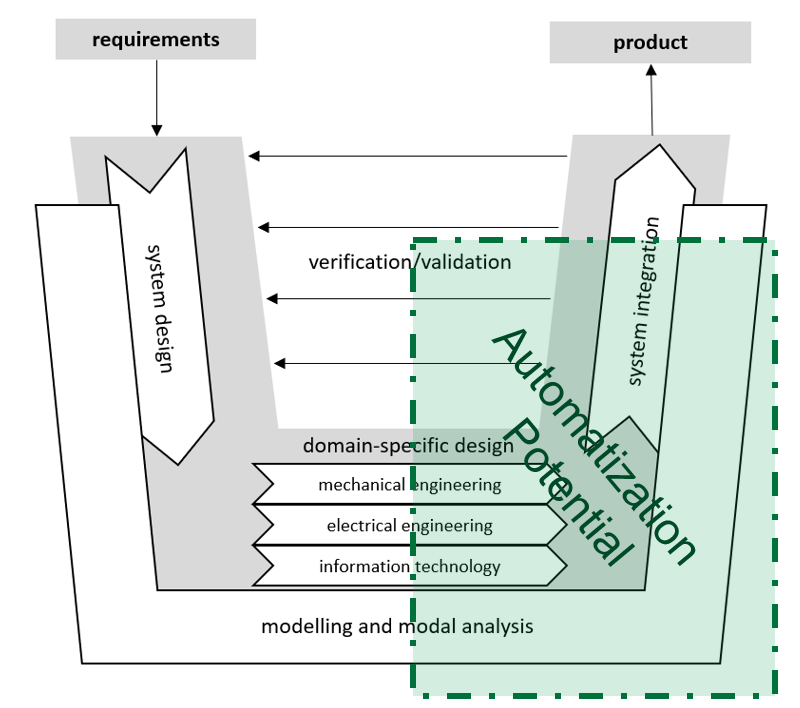
\includegraphics[scale=0.6]{pics/VDI_2206.PNG}
    \caption{\label{pic:VDI2206} Automatization potential in the VDI 2206 Guideline \cite{Jansch2006THEDO}.}
\end{figure}\\
Another issue which can arise in designing processes is the amount of optimization work, which takes a major part of the development time in high efficient products.
Optimization therefore stretches, from topology optimization, to variants comparison and parameter tuning \cite{hornby_automated_2006, khalafallah_electimize_2011, evans_aerodynamic_2017, slagter_perform_2020}. 
This lead to an extraordinary potential for time saving in lightweight design, as shown in Figure \ref{pic:VDI2206}.\\
Assuming that complex multi-disciplinary systems can be modelled sufficiently, the question of how to find the optimal solution arises.
Therefore, an algorithm has been developed, which requires the minimal amount of system knowledge.
Algorithms like simulated annealing \cite{khachaturyan_thermodynamic_1981}, 
evolutionary algorithm \cite{wu_ensemble_2019}, particle swarm optimization \cite{Kennedy1995} and Bayesian optimization \cite{marcuk_optimization_1975}
are the most popular ones, by have proven to find the global optimum and not to fall in local minima.\\
Following the state of the art, this paper wants to introduce an open-source information based workflow engine for design processes.
The proposed work will therefore focus on the representation of complex multi-domain tasks and implements optimization techniques to find the best product for a custom use case.